\begin{frame}
    \frametitle{\problemtitle}

    \begin{columns}
        \begin{column}[T]{.75\textwidth}
            \begin{itemize}
                \item Determine the \emph{convincingness} of each of $1 \leq n \leq 2 \cdot 10^5$ suspects.
                \item For every suspect, you know the time at which they arrived
                    at the scene and the duration they stayed
                ($1 \leq a,t \leq 10^9$).
                \item A suspect $A$ provides an alibi for suspect $B$ if and only if
                $A$ was in the room for the entire duration $B$ was in there.
                \item A suspect without an alibi has convincingness $0$.
                Otherwise, their convincingness is $1$ more than the convincingness of the most convincing suspect
                who provides them with an alibi.
            \end{itemize}

        \end{column}

        \illustration{.2}{rob}{Rob. Pixabay License by Henning on \href{https://pixabay.com/de/illustrations/hacker-hacking-diebstahl-cyber-5027679/}{Pixabay}}%
    \end{columns}

    \centering
    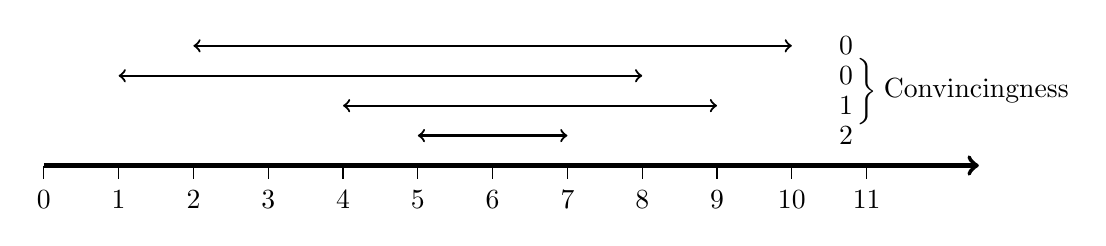
\begin{tikzpicture}[scale=0.95]
        \usetikzlibrary{calc}

        \foreach \x in {0,1,2,...,11}{
            \coordinate (A\x) at ($(0,0)+(\x*1cm,0)$) {};
            \draw ($(A\x)$) -- ($(A\x)-(0,5pt)$);
            \node at ($(A\x)+(0,-3ex)$) {\x};
        }
        \draw[ultra thick,arrows=->] (A0) -- (A11) -- ($(A11)+1.5*(1,0)$);

        \draw[<->,thick] (2,1.6) -- (10,1.6);
        \draw[<->,thick] (1,1.2) -- (8,1.2);
        \draw[<->,thick] (4,0.8) -- (9,0.8);
        \draw[<->,thick] (5,0.4) -- (7,0.4);

        \node[anchor=west] at (10.5,1.6) {0};
        \node[anchor=west] at (10.5,1.2) {0};
        \node[anchor=west] at (10.5,0.8) {1};
        \node[anchor=west] at (10.5,0.4) {2};

        \node[anchor=west] at (10.73,1) {\huge$\Bigg\}$};
        \node[anchor=west] at (11.1,1) {Convincingness};
    \end{tikzpicture}

    \small
    Illustration of Sample Input 1.
\end{frame}
